\documentclass{sigchi-ext}
% Please be sure that you have the dependencies (i.e., additional
% LaTeX packages) to compile this example.
\usepackage[T1]{fontenc}
\usepackage{textcomp}
\usepackage[scaled=.92]{helvet} % for proper fonts
\usepackage{graphicx} % for EPS use the graphics package instead
\usepackage{balance}  % for useful for balancing the last columns
\usepackage{booktabs} % for pretty table rules
\usepackage{ccicons}  % for Creative Commons citation icons
\usepackage{ragged2e} % for tighter hyphenation
\usepackage{float}
\usepackage{pgfgantt}
\usepackage{pgfgantt-custom}
\usepackage{verbatim}
\usepackage{gensymb} % for ohm-symbol
\usepackage{todonotes}

% For gifs?
\usepackage{animate}

% \usepackage{marginnote} \usepackage[shortlabels]{enumitem}
% \usepackage{paralist}

%% EXAMPLE BEGIN -- HOW TO OVERRIDE THE DEFAULT COPYRIGHT STRIP --
 \copyrightinfo{\vspace*{-20pt}
\includegraphics{figures/paperCredits1}}
%% EXAMPLE END

\title{GUARDIAN SUIT: Baby monitoring onesie using eTextile}

\numberofauthors{3}
% Notice how author names are alternately typesetted to appear ordered
% in 2-column format; i.e., the first 4 authors on the first column and
% the other 4 authors on the second column. Actually, it's up to you to
% strictly adhere to this author notation.
\author{%
  \alignauthor{%
    \textbf{Madrigal N. Totayo}\\
    \affaddr{University of Copenhagen} \\
    \affaddr{Universitetsparken 5} \\
    \affaddr{2100 Copenhagen} \\
    \affaddr{vnw888@alumni.ku.dk} } \vfil \alignauthor{%
    \textbf{Mark Wulff}\\
    \affaddr{University of Copenhagen}\\
    \affaddr{Universitetsparken 5}\\
    \affaddr{2100 Copenhagen} \\
    \email{lrh211@alumni.ku.dk} }  \vfil \alignauthor{%
    \textbf{Mark J. Jacobi}\\
    \affaddr{University of Copenhagen}\\
    \affaddr{Universitetsparken 5}\\
    \affaddr{2100 Copenhagen} \\
    \email{dcz738@alumni.ku.dk} } }

% Paper metadata (use plain text, for PDF inclusion and later
% re-using, if desired)
\def\plaintitle{SIGCHI Extended Abstracts Sample File: Note Initial
  Caps} \def\plainauthor{First Author, Second Author, Third Author,
  Fourth Author, Fifth Author, Sixth Author}
\def\plainkeywords{SIDS; eTextile; monitoring; breathing; lying position.}
\def\plaingeneralterms{Documentation, Standardization}

%% Set up our PDF with metadata
\hypersetup{%
  pdftitle={\plaintitle}, pdfauthor={\plainauthor},
  pdfkeywords={\plainkeywords}, }

% \reversemarginpar%

\begin{document}
\pagenumbering{arabic}
\maketitle

% Uncomment to disable hyphenation (not recommended)
% https://twitter.com/anjirokhan/status/546046683331973120
\RaggedRight{}

% Do not change the page size or page settings.
\begin{abstract}
This project involves using eTextiles to make a modified onesie for infants to monitor their health and well-being during sleep.
Using different types of eTextile, we made Guardian Suit which can detect the lying position and breathing of an infant. 
Though the lying position detection works well, the breathing sensor does not perform to our expectations, and we therefore recommend 
further research beyond our approach.\todo{I dont really know, but does this seem ok? (please alter it if you have a better phrasing or
perhaps with more "concrete" results showcase)}

\begin{comment}
  The most important rule of Abstracts is that they describe the work, not the paper. Include, at most, one sentence of motivation. Save the rest of your motivation for the Introduction. Effective Abstracts focus on two things: (1) Describing what was done. (2) Describing what was found (key results). Be specific about your key findings. Instead of "many" say "84\%". Keep the Abstract to one paragraph and fewer than 200 words.
\end{comment}
\end{abstract}

\keywords{\plainkeywords}

\category{J.3}{Health and Medical systems}{Medical information systems}
% See http://www.acm.org/about/class/ccs98-html for all (men denne er den eneste som passer til os)

\section{Introduction}
Parents and guardians are often worried about the infants health and well-being. Because of this, various infant monitoring technologies have been developed. These monitoring devices checks the sleeping environment for the infant (e.g. critical shifts in the temperature of the room), and usually requires an object being present near the infant's crib, which we find to be rather clunky. Unfortunately, they do not give any information on which position the infant is lying in and whether it is breathing or not.

Many recommendations for the infants sleeping positions and environments have been made in order to lower the probability of Sudden Infant Death Syndrome (SIDS)\footnote{\url{https://en.wikipedia.org/wiki/Sudden_infant_death_syndrome}}.
%\begin{comment}
\marginpar{%
  \vspace{-20pt} \fbox{%
    \begin{minipage}{0.925\marginparwidth}
    \textbf{Guardian Suit} \\
      \begin{figure} [H]
    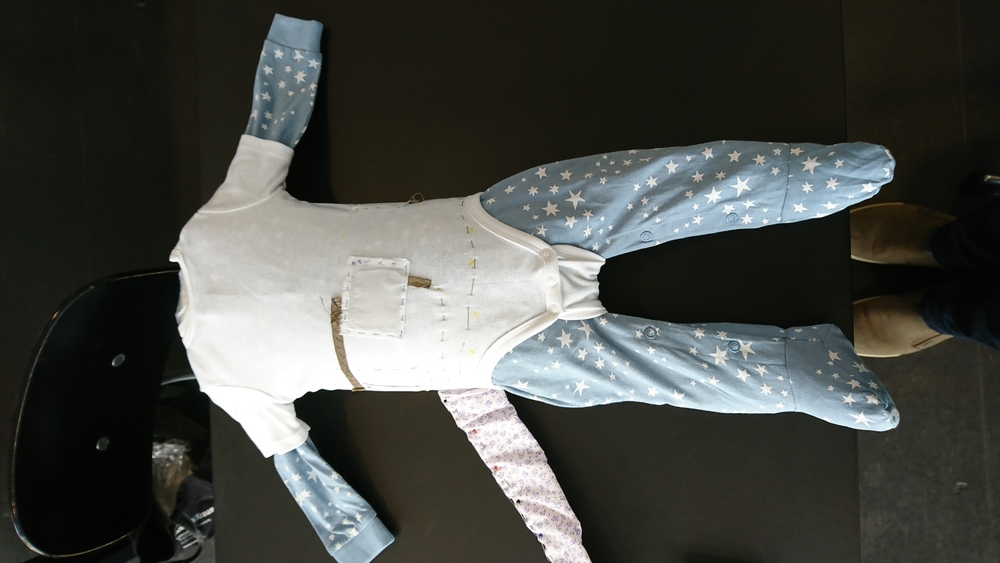
\includegraphics[width=1.5\textwidth,angle=-90]{img/guardian_suit_final}
    \centering
    \caption{The Guardian Suit (onesie - no breathing sensor as we need it separately to test it).}
\end{figure}
      \begin{figure} [H]
    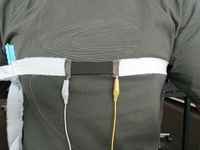
\includegraphics[width=1.0\textwidth]{img/breathing_sensor_final}
    \caption{The breathing sensor, mounted on a strip of cotton fabric for testing.}
\end{figure}
    \end{minipage}}\label{sec:sidebar} }
%\end{comment}
After years of research by the American Academy of Pediatrics (AAP) \cite{aap-1992,aap-1996,aap-2005} the main recommendations for minimizing the probability of SIDS is to detect (1) whether the infant is breathing or not, and (2) when the infant changes position. To address the recommendations we developed Guardian Suit, a onesie with one-dimensional textile sensors sewn (3) around the chest area, (4) on the lower-back, (5) stomach, and (6) one on each side.

The first sensor introduced (3) consists of piezoresistive elastic polymer, conductive
nylon and conductive thread which decrease in resistance when stretched. This allows for detecting whether
the infant is breathing or not. The sensors for the back, stomach and sides (4, 5, 6) consist of pieces of conductive nylon, conductive thread, and non-elastic piezoresistive fabric in-between two pieces of conductive fabrics. They decrease in resistance when pressure is applied to them. 
These sensors are placed as such, in order to detect whether the infant is in a
prone (i.e. on the stomach), supine (i.e. on the back) or lateral (i.e. on the
side) position.

% Ville forklare noget om isolering af de ledende stoffer, men vi kan også bare fjerne det
\begin{comment}
Furthermore, as our product is electrical, we don't want the possibility of
hurting the baby e.g. by getting electrocuted. For this, we created strips out
of conductive fabric that were sewn into the onesie. 
These are then connected to the development board by crimping the
sensors\footnote{\url{https://www.pololu.com/product/1928\#lightbox-picture0J3280;main-pictures}} or by using
snaps\footnote{\url{https://www.sparkfun.com/products/11347}}.
\end{comment}

To test this crude first generation prototype, we manufactured a doll which 
mimic some properties of a baby, i.e. weight and shape. We put the Guardian Suit
on the doll and moved it into various positions. We found that the pressure pads
worked very well in detecting the positioning of the doll.\todo{Mark J. 
forklar resultater for pressure test ting her kort og "erroren" vi oplevede (25 gange hver side ting)}\\
As for the breathing
sensor, we tested it on ourselves as we did not have access to a baby. Though
it was able to detect breathing, the very subtle stretch in the piezoresistive
elastic polymer is hard to detect and any body movement would overshadow the output
from breathing. However, it still was possible to produce a curve from which 
we are able to identify breaths.\\
With continuous use the material becomes lax as the nylon does not maintain its stretch
property. We found that continuous use for more than 30 minutes made the material
too lax to determine breathing as accurately as in the beginning of usage.

% Ved ikke rigtigt hvordan det skal formuleres alligevel
In the following, we will describe how we constructed
the breathing and pressure sensors, how we evaluated
these and how they will be integrated into Guardian Suit.\\
We also provide some material evaluation of the Eeontex
piezoresistive stretch fabric regarding the resistance
change when stretched.

% CONTRIBUTIONS:
% 1. material evaluation of Eeontex stretch fabric
% 2. prototype: Guardian Suit (breathing sensor and pressure sensor onesie)
\begin{comment}
In the following, we will describe our findings of how the 
prototype should be used. Thus, we had to build it with the following in mind: (1) sensor construction and placement techniques, (2) connecting the sensors to the development board without the use of wires, and (3) usage scenarios and possible feedback from the readings.
\end{comment}

\begin{comment}
% Fjernet fordi Kasper føler det er fortalt i introduktionen (som skal rettes til)
\section{Guardian Suit}
% first paragraph should be rephrased
% for the final submission
Guardian Suit consists of three key components which
makes up the prototype. The breathing sensor which is
made from Eeontex piezoresistive elastic fabric, conductive
nylon and conductive thread. Pressure sensors made
from conductive fabric, Eeontex piezoresistive (non-elastic)
fabric, conductive nylon and conductive thread. Software
processing of the output data from the sensors.

The components are embedded into a regular cotton baby
onesie. Guardian Suit will thereby monitor the baby
directly, oppose to our conventional baby monitors which 
focuses more on the baby's environment with sound and video.
\end{comment}

% comment for at kunne fjerne fra dokument
\begin{comment}
\colorbox{cyan}{Modified universal onesie bought from a generic baby clothing store}
\colorbox{cyan}{Arguments for why this is a
better approach: Affordable, non-intrusive?}
\colorbox{cyan}{Picture overview}
\colorbox{cyan}{key components}
\end{comment}

\section{Motivational scenario}
The parents of an infant realizes that it is dozing off, and decides to put the infant in a crib for a nap, where the infant is dressed with the Guardian Suit beforehand. The infant is initially placed on its back in the crib, and the parents goes about with their work. Whenever the infant changes position, either to one of the sides or on the stomach, the parents are notified by the pressure pads embedded in the suit in order to take action. The same with the breathing sensor, when the infant isn't breathing 20-44 consecutive breaths per minute \cite{a18-huang}, the parents are notified, and thus, can take immediate action.

\section{Related work}
Many products have been developed to allow parents and guardians to monitor their infants. One of them is the Georgia Tech Wearable Motherboard (GTWM)\footnote{\url{http://www.gtwm.gatech.edu/}}. Initially developed in collaboration with the US Navy Department to monitor a soldier's vital signs by detecting the penetration of e.g. bullets and shrapnel, it was later augmented to monitor an infant's breathing or heart rate by using cardiorespiratory sensors on a vinyl strap, as described by Fantauzzacoffin et al. \cite{p285-fantauzzacoffin}. The engineers had created it by weaving signal transmission lines and integrated the sensors into a onesie. One mother didn't mind her infant to be surrounded by wires from the device, and found it to be quite comfortable.

Kroutil et al. \cite{a33-kroutil} used electrically conductive stranded yarn as sensors, placed underneath the lower bed sheet to detect respiration among individuals. The sensors measured the respiratory activity by the alteration of electrical capacitance of the chest area. This was done so one could monitor patients respiration without inconveniencing them with wiring and sensors attached to their bodies.

Another bedsheet monitor was proposed by Huang et al. \cite{a18-huang}. Embedded with pressure sensors and in conjunction with collated data, they were able to detect whether the person was breathing or not within a certain time interval, corresponding to a predetermined minimum breathing rate.

Even though creating the sensors within the fabric of the surface the infant is lying on during sleep has produced satisfactory results \cite{a18-huang, a33-kroutil}, we have chosen another approach. Guardian Suit combines the wearability, comfort, and ease of use of GTWM\footnote{\url{http://www.gtwm.gatech.edu/}} \cite{p285-fantauzzacoffin} with the pressure sensing technologies used in the bedding solutions. We receive feedback whenever the infant is in either position i.e. prone (stomach), supine (back) or lateral (side). With the electrical elastic polymer we are able to detect the breathing rate of the baby. Finally, with constraints as proposed by Huang et al. \cite{a18-huang}, we can detect whenever any individual is in a critical state.

We are using piezoresistive conductive
stretchable fabric for breathing detection. However, an alternative solution method to the breathing sensor
could be investigated based on the research of Vogl et al. \cite{stretcheband}, who
tested various stitching patterns of conductive thread and the resistance measured
when stretched.

\clearpage

\section{Technical evaluation of materials/sensors}

\subsection{EeonTex piezoresistive elastic polymer}

%\begin{comment}
\marginpar{%
  \vspace{-10pt} \fbox{%
    \begin{minipage}{0.925\marginparwidth}
    \textbf{Piezoresistive elastic polymer evaluation} \\
      \begin{figure} [H]
    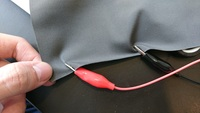
\includegraphics[width=1.0\textwidth]{img/resize/w200/breathing_sensor}
    \caption{Test of the piezoresistive elastic polymer using crocodile clip wires.}
\end{figure}
      \begin{figure} [H]
    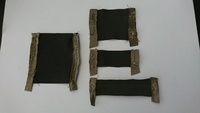
\includegraphics[width=1.0\textwidth]{img/resize/w200/stretch_sensors}
    \caption{The different sizes of stretch sensors we tested (missing 1.0x5.0cm)}
\end{figure}
      \begin{figure} [H]
    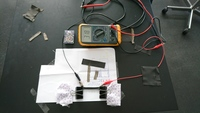
\includegraphics[width=1.0\textwidth]{img/resize/w200/stretch_test_setup}
    \caption{Test setup for the stretch sensors, results in table \ref{tab:stretch-test}}
\end{figure}
    \end{minipage}}\label{sec:sidebar} }
%\end{comment}

For the breathing sensor we will use the EeonTex piezoresistive elastic polymer.
This polymer has the property that the resistance is decreased when the fabric
is stretched.

From the consultation of some eTextile experts, we determined
that tuning the sensor will be a three step approach.\\
First, we will find the piece size of the material which
is the most sensitive given the limited size we need it to be
to fit on the chest. Next, we will experiment with various
resistors to find the best suitable one for our input range.
Thirdly, configure the smoothing software for the sensor readings.

As we need some indication of the amount the material will
be stretched, we measured the circumference of the chest
when fully exhaled, fully inhaled and a regular breath
(this will vary depending on the person).
\begin{table}[H]
  \centering
  \begin{tabular}{l r r}
    % \toprule
    & \multicolumn{1}{r}{\small{\textbf{Breath circumference measure}}} \\
    \cmidrule(r){2-3}
    {\small\textit{State}}
    & {\small \textit{circumference (cm)}}
    & {\small \textit{Change (cm)}}\\
    \midrule
    Full exhale    & 101.0 & \\
    Full inhale    & 107.0 & 6\\
    Regular exhale & 104.2 & \\
    Regular inhale & 105.5 & 1.3 \\
    % \bottomrule
  \end{tabular}
  \caption{Measurements of chest circumference when breathing. Used for testing the Eeontex material.}~\label{tab:circumference}
\end{table}
From the above table we get an idea of how much a single breath affects the circumference
in an adult male. Though this is not representative of a baby, due to the
inaccessibility of one and that we want to develop a first iteration prototype, this
will be our basis of the breathing sensor.

We see that the difference in a full forced inhale/exhale is about 6 cm. whereas regular
breathing only results in around 1 cm in difference.\\
We have experimented with the different sizes of the Eeontex conductive piezoresistive
stretch fabric. From the breath circumference table we can see the change varies in cm and construct a simple experiment in order to evaluate the change in resistance given
different fabric sizes, as noted in the table below.
\begin{table}[H]
  \centering
  \begin{tabular}{l r r r r}
    % \toprule
    & \multicolumn{4}{l}{\small{\textbf{Stretch sensor test results}}} \\
    \cmidrule(r){2-4}
    {\small\textit{Size (cm x cm)}}
    & {\small \textit{+0.0cm}}
    & {\small \textit{+0.5cm}}
    & {\small \textit{+1.0cm}}
    & {\small \textit{+1.5cm}} \\
    \midrule
    1.0x5.0    & 306 & 241(~79\%) & 217(~71\%) & 202(~66\%)\\
    2.5x5.0    & 101 & 78(~77\%)  & 63(~62\%)  & 58(~57\%) \\
    2.5x7.5    & 122 & 108(~89\%) & 89(~73\%)  & 83(~68\%) \\
    5.0x5.0    & 63  & 53(~81\%)  & 39(~62\%)  & 37(~59\%) \\
    5.0x7.5    & 44  & 47(~107\%)  & 39(~89\%)  & 35(~80\%) \\
    % \bottomrule
  \end{tabular}
  \caption{Resistance measured using volt-meter in k$\Omega$}~\label{tab:stretch-test}
\end{table}
We performed the test with two sets of the material sizes.
We discovered during the first test that if the material
is stretched beyond a certain limit, the material gets
damaged such the piezoresistive property changes. In our case,
we found that it becomes less sensitive.

From the experimentation, we have determined the 2.5x5.0cm size
performed the best and therefore we will proceed with this
configuration.

\clearpage

\subsection{Pressure sensors}
The position sensors will be eTextile pressure sensors by putting two conductive
fabrics with a piezoresistive fabric in-between which changes resistance when
pressed.

For testing
the efficiency of the sensor, we started by making a
simple prototype before the actual sensors.
We used some copper wires as connectors, 1.4 mm, after verifying the pad with
crocodile clip wires. When we tested the pad, the idle resistance measured when on the table was
around 900 (due to fabric deformities this would vary). by slight touch, the resistance dropped to around 400. From this observation we determined that 
this type of pad would suffice as pressure sensor.

%\begin{comment}
\marginpar{%
  \vspace{-160pt} \fbox{%
    \begin{minipage}{0.925\marginparwidth}
    \textbf{Pressure sensor evaluation} \\
      \begin{figure} [H]
   \centering 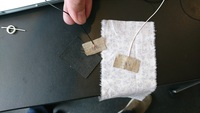
\includegraphics[width=0.85\textwidth]{img/resize/w200/pressure_sensor.jpg}
    \caption{The prototyping of the eTextile pressure sensor pad.}
\end{figure}
      \begin{figure} [H]
   \centering 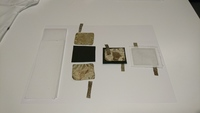
\includegraphics[width=0.85\textwidth]{img/resize/w200/pressure_sensor2.JPG}
    \caption{Overview of the final pressure sensor pad construction (materials and assembly).}
\end{figure}
      \begin{figure} [H]
   \centering 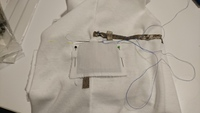
\includegraphics[width=0.85\textwidth]{img/resize/w200/pe_integration.JPG}
    \caption{Pressure sensor sewn into Guardian Suit.}
\end{figure}
    \end{minipage}}\label{sec:sidebar3} }
%\end{comment}

Construction of the sensors embedded into Guardian Suit, we used 
silver plated nylon and conductive thread (coated with micron-thick layer of 
natural silver). As we want to demonstrate that all materials used can be
composed of eTextiles, we chose this over copper wiring.

When constructing the pads, all the conductive fabrics (non stretch) were
burned around the edges to keep the fabric from fraying.
For wrapping and keeping in place, we used a thin cotton
fabric which is non-conductive and kept together using
fabric glue.
For connectors we use the silver plated nylon fabric to make a stripe around
the stomach area for the main connector which all pads will be connected to.

For the wiring of each of the analog input to each pad, we used conductive
thread. In our prototype the thread leads out of the onesie by a line of
fabric to make it less restrictive when manipulating the doll which it is
put on. However, as future work the microcontroller would be embedded into
the onesie as well and use wireless connectivity to transmit data.

To evaluate the pads which will be embedded into Guardian Suit, we applied 
increasing weights and measured the resistance using a volt meter.\\
As we did not have weights we used danish coins, 20 and 5 kr. coins, which both
weigh (sampled using 5 coins) 9.3g each. Therefore we can treat each of them as
being the same weight.
\begin{figure} [H]
   \centering 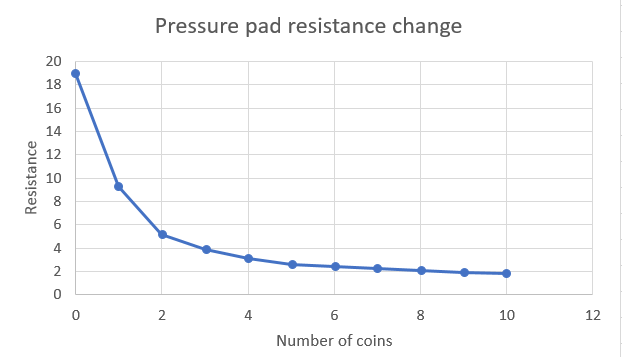
\includegraphics[width=0.45\textwidth]{img/chart.PNG}
    \caption{Resistance change by weight (k$\Omega$)}
\end{figure}
From the chart we can see that around 100g of force will drop the resistance
by around 90\%. From these results we determined that the sensors would be suitable
as a newborn weighs on average 3.5kg.

\clearpage

\section{Prototype construction}
What separates Guardian Suit from conventional alternative baby monitors 
(e.g. cameras and noise sensors) is its relative low cost and monitors the
baby directly and not the environment around it. The 
sensors are not difficult to produce and can be integrated into any fabric-based
onesie by sewing. The only significant component in Guardian Suit is the
micro-controller which would be embedded into the onesie also.\\
To construct the prototype we made the sensors and evaluated them as
described in the precious sections. Then we bought a cotton leg and arm-less
onesie from H\&M and embedded our sensors into it.

For connectors, we used silver plated nylon and conductive thread (coated with
micron-thick layer of natural silver. We also evaluated these against copper
wiring in the pressure sensor evaluation section. The issue with these
connectors is that because they are plated with silver, washing prototype
would over time reduce the conductivity of the material.

The prototype itself consists of the 4 pressure sensors, and one breathing sensor. 
An Arduino MKR1000 micro controller reads the resistance of the sensors and transmits the raw values over an USB connection to a computer. The computer then represents the raw sensor data as graphs.

The Arduino micro controller is hooked up to a pull-up resistance circuit, as shown on \autoref{fig:ardcirc}. The pull-up circuit makes the voltage change on the terminals \textbf{A0} to \textbf{A4}, when the sensors resistance change. 
The micro controller compares the input voltage on the terminals to the reference voltage defined in the system. The reference voltage is set externally by potentiometer as illustrated on the circuit diagram (\textbf{Aref}). This gives us granular control of the sensor readings. This is helpful for illustrating small fluctuations in the voltage. The breathing sensor has a very low actuation distance, and therefore low fluctuations. Changing the reference voltage will therefore make it easier to detect changes.  
\colorbox{cyan}{Add to conclusion?}.

\begin{figure} [H]
   \centering 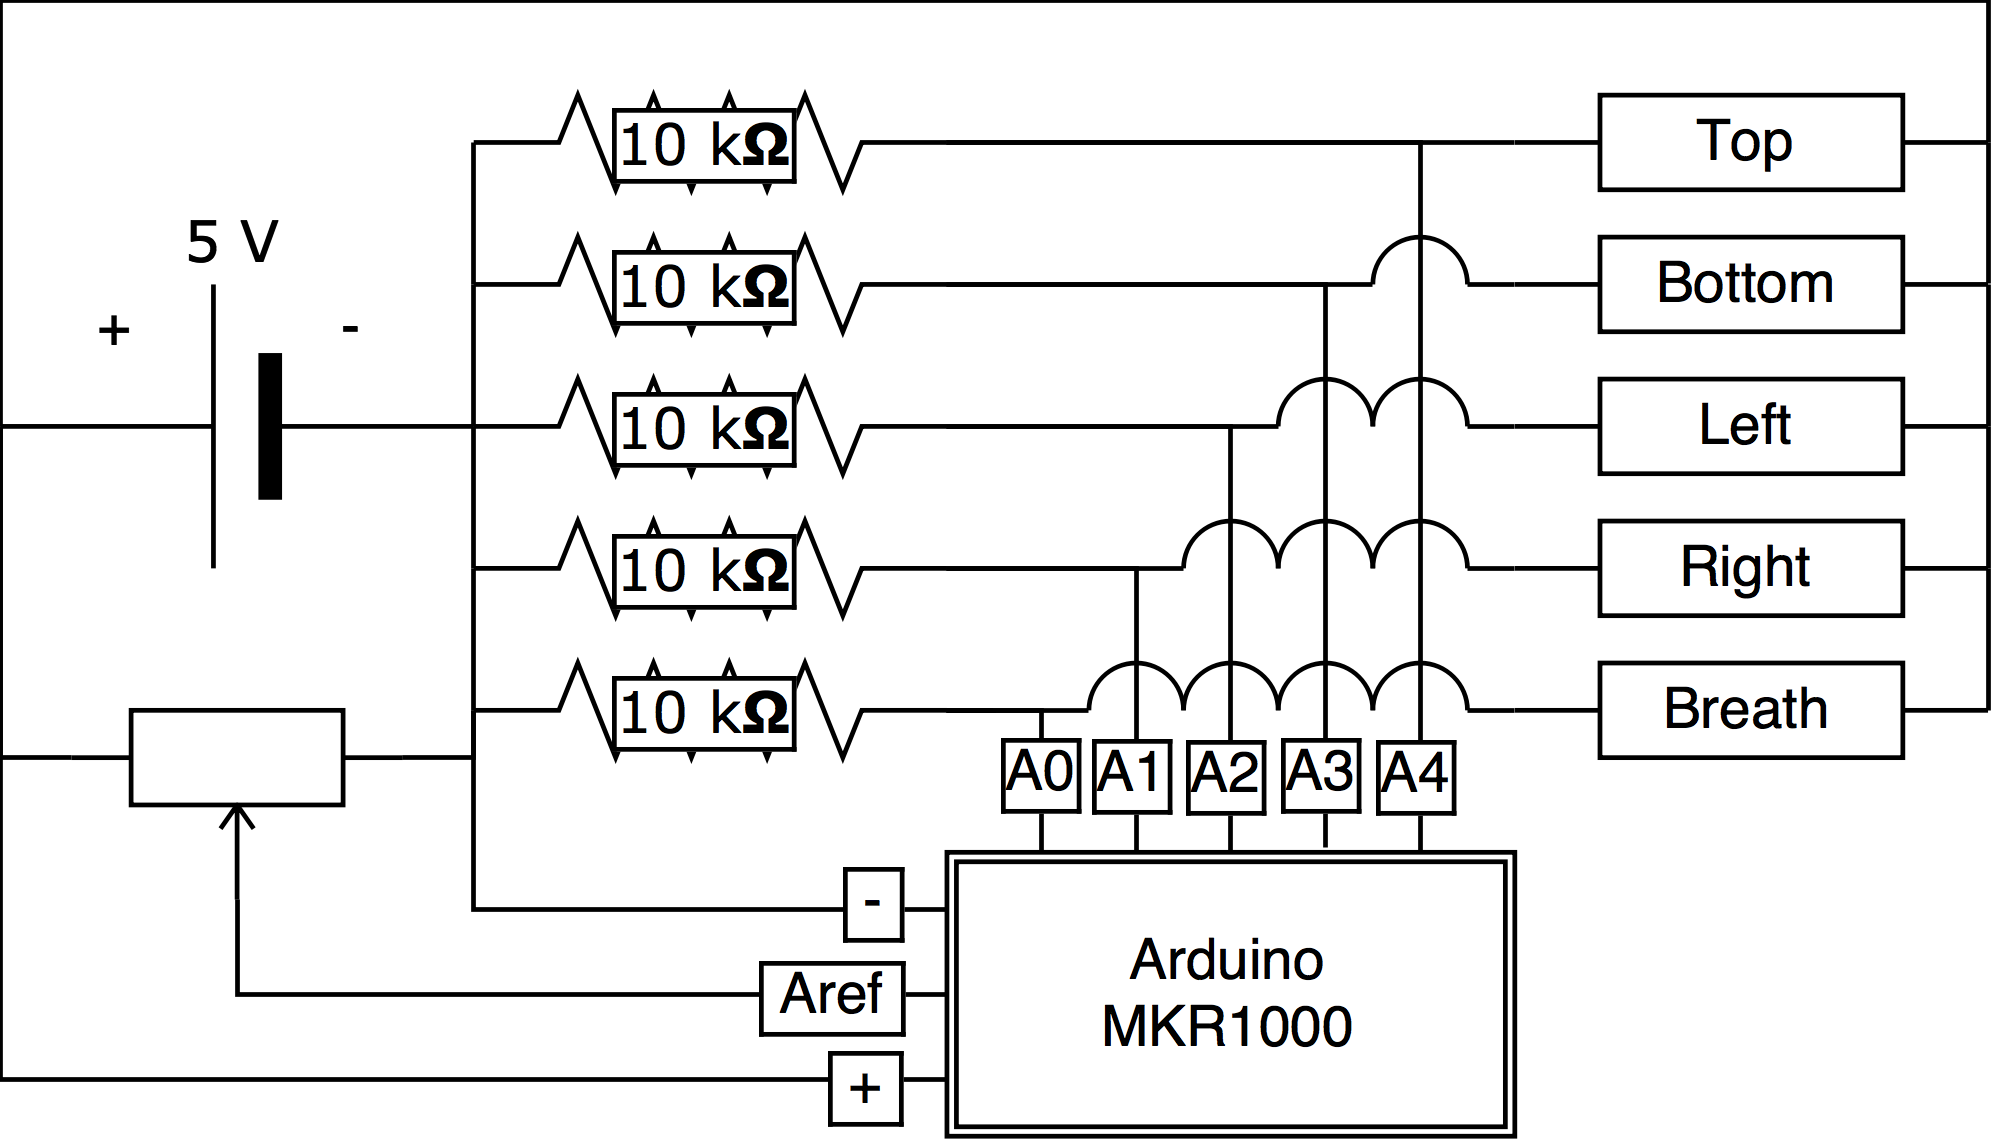
\includegraphics[width=0.45\textwidth]{img/arduino_diagram}
    \caption{Circuit diagram of the sensor setup}
    \label{fig:ardcirc}
\end{figure}

The micro controller applies a low pass filter before sending the data to the computer. The low pass filter is based on the last $n$ values read, where each values gets replaced after $n$ iterations. $B$ is the buffer(last values read), and $D$ is the current readings. $k$ is the current iteration.
$$
V_k= \sum\limits_{i=1}^n 
\left\{
\begin{array}{ll}
    k \bmod n = i & B_k = D_k\\
    else          & B_k
\end{array}\right\}\frac{1}{n}
$$
This illustrates that the average is taken over the $n$ iterations, and once per iteration a buffer value is changed, "round robin" style.


\colorbox{cyan}{Add image see comments}.
%
% Add image of the graphing program running
%
%\begin{figure} [H]
%   \centering 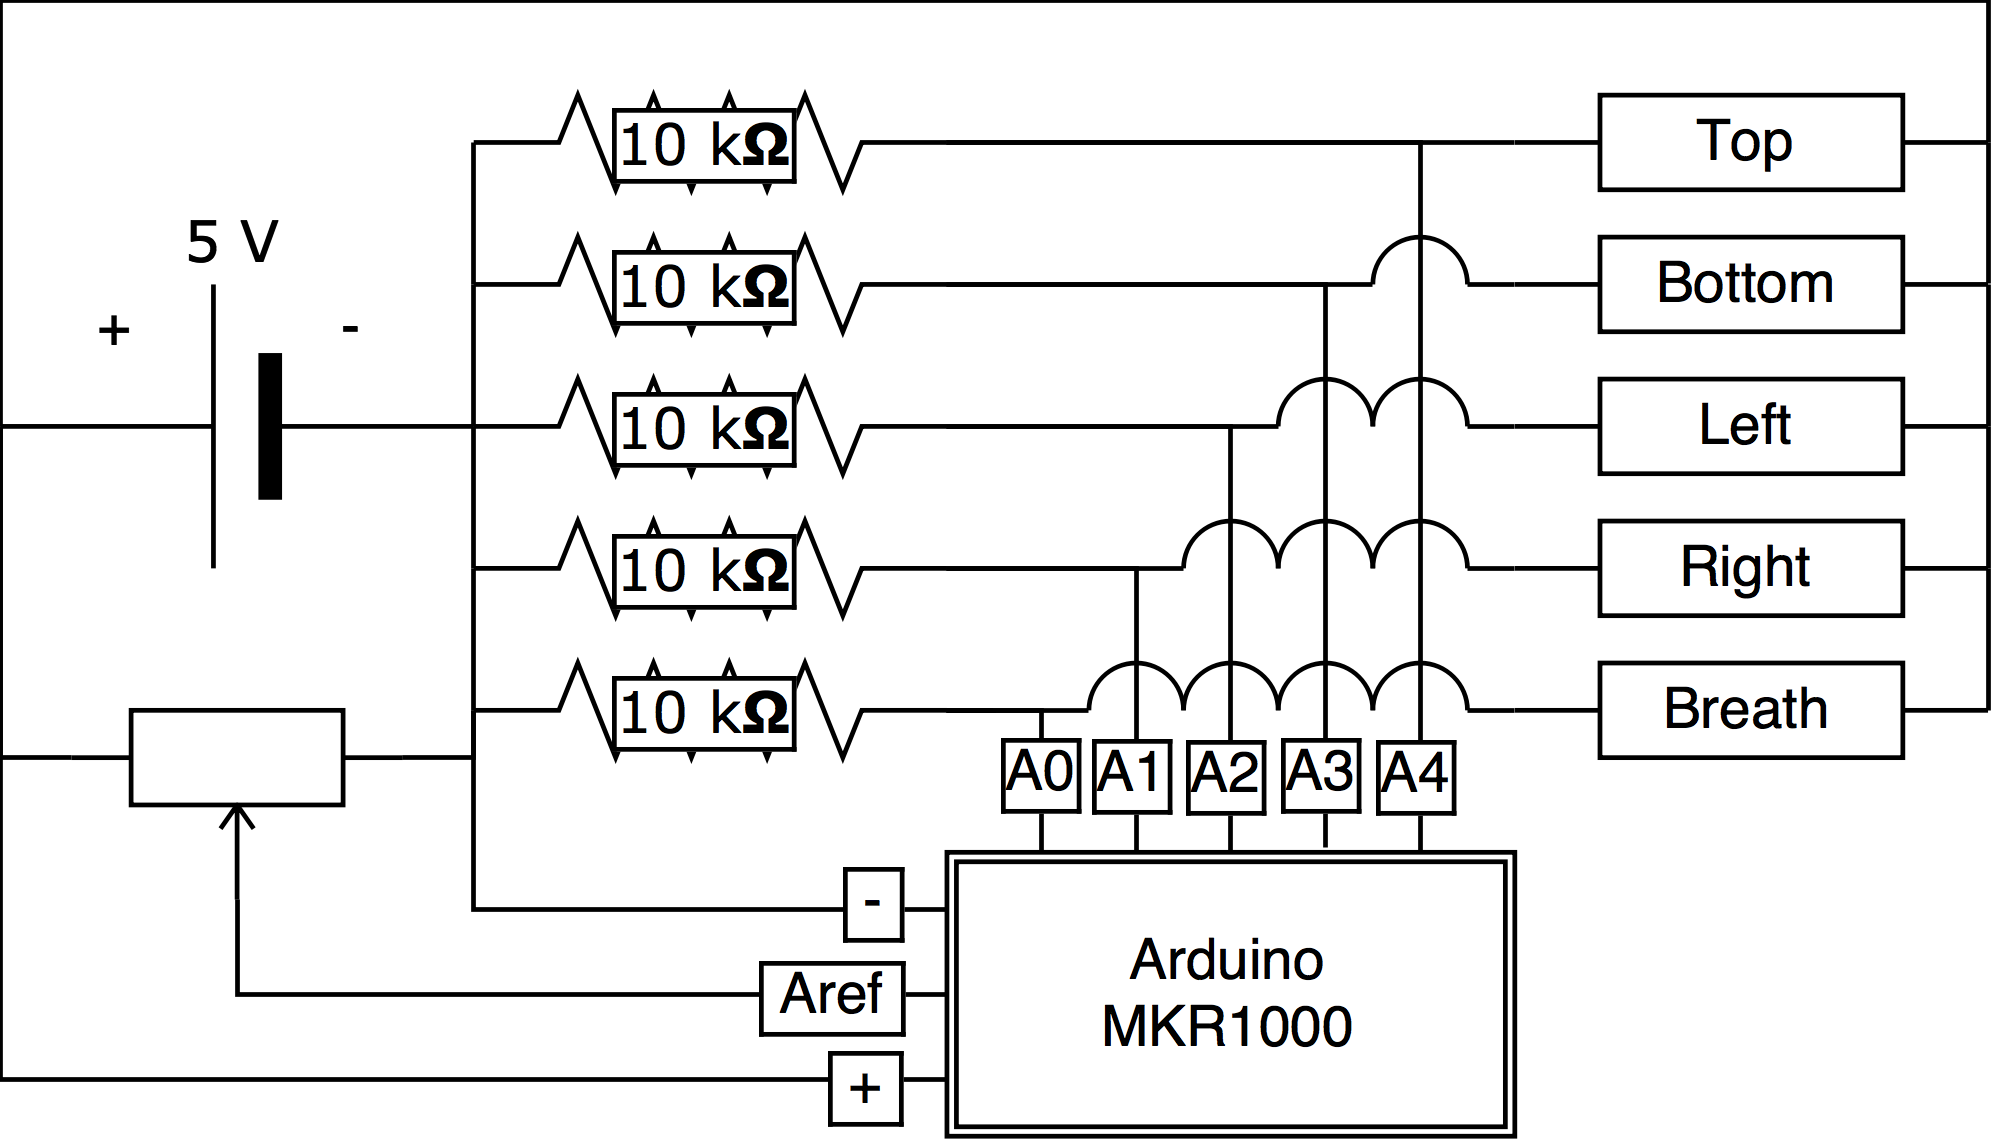
\includegraphics[width=0.45\textwidth]{img/arduino_diagram}
%    \caption{Circuit diagram of the sensor setup}
%\end{figure}

When the sensor data has been processed, the data is ready to be sent to the computer. A python program reads the data, and represents it on the screen.
The first column contains the individual sensor data. The graph is time based, where the range is set to the highest and lowest observed value, taken from a timespan of 5 seconds.
The bottom column contains the same timespan, but shows all the sensor values at once, with a fixed range from $0$ to $1023$.


\section{Prototype evaluation}
%\begin{comment}
\marginpar{%
  \vspace{-85pt} \fbox{%
    \begin{minipage}{0.925\marginparwidth}
    \textbf{Prototype evaluation} \\
      \begin{figure} [H]
   \centering \animategraphics[loop,autoplay,width=1\linewidth,poster=70]{12}{breathing_sensor/breathing-}{0}{220}
    \caption{Breathing sensor evaluation test.}
    \label{fig:breath_eval}
\end{figure}
    \end{minipage}}\label{sec:sidebar4} }
%\end{comment}

Without using an actual baby for testing, we created a
doll consisting of rice and flour to represent an
approximation of a baby's weight and size. The amount we 
can test using this doll is limited, however, we are able 
to conduct a very technical evaluation of the pressure 
would work in general.

We put Guardian Suit on the doll and placed it in various
positions to verify the actuation of the pressure sensors.
As observed like in the technical evaluation of the sensors,
the pressure of the doll's around 3kg of distributed weight
is able to actuate the sensors clearly when lying on one. 
Some of the sensors did show slight actuation due to the
bending of the sensor because of the doll's shape. However,
it was clear to see when the doll was lying on one as the 
resistance decreased much more.\todo{Mark J. Write thing about pressure sensor testing here - beautiful diagrams}

For the breathing sensor we sew the breathing sensor into
a long strip of cotton fabric to be able to adjust the 
sensor around an adult. We tried the sensor on an 
adult male in order to verify the ability to identify 
breaths.\\
Generally as mentioned earlier, breaths are very subtle and
overshadowed by muscle flex. However, when completely still,
the sensor is able to detect breaths. As depicted in the figure \ref{fig:breath_eval},
we can clearly identify breaths as the peaks on the graph, and exhale as
the drop.\\
However, though this works in this isolated case, when using the breathing sensor
over longer periods of time, the fabric becomes more and more lax. We 
tried continues usage for around 30 minutes and observed this behaviour. This causes the resistance
change to become more prone to error as the noise becomes more prominent. From this, we speculate
that this material might not be well suited for our breathing sensor or other constructions which
requires the continues interaction with the material.

\section{Future work}
We used piezoresistive elastic polymer for our breathing sensor. Using this,
we were able to detect breathing but with very limited signal. Also, flexing the muscles
would produce much more prominent signals. We don't expect this to be any
different given any other materials or stretch sensors. However,
based on the research of Vogl et al. \cite{stretcheband} it would be interesting
to see which signal is produced when making the same kind of stitch pattern on
the test area and evaluate the signal output.

The Guardian Suit works by the test on the doll in the study. However,
the prototype has yet to be evaluated on an actual baby which would provide the
most accurate real world usage as the product is intended for babies. However,
another place to start would be to build it into an adult size piece of clothing
and try it on an adult.

Generally, the prototype can be further developed in multiple ways. One would be to 
find a micro-controller to be embedded into the onesie. Also, given the connectors currently are just
sewn into the onesie, finding a way to insulate them would be something to consider in a future
iteration of the prototype.

\section{Conclusion and discussion}\todo{check report with the "trick", you should be able to summarize each paragraf with a single sentence. (see first paragraph for example)}
We set out, trying to create a more direct monitoring solution for infants. Our solution, Guardian Suit, was 
modifying a onesie by embedding pressure sensors made from eTextile and a breathing sensor around the
chest, also using eTextile. From these sensors we are able to obtain output which will enable us to 
detect the lying position of the infant and the breathing rate.\todo{example: We created Guardian Suit using eTextile
to help monitor infants. (I think this is correct)}

Detecting the lying position of the infant using pressure sensors made from eTextile was very reliable from our limited amount of 
testing using the doll made from flour and rice. However, though we obtained accurate readings from the doll, this does not 
reflect a real infant as they vary in size and fat. Therefore it is not possible to conclude that this solution is a definite viable
solution, though it is interesting to proceed with infant trails.\todo{ohm... other or better formulation?}

The breathing sensor made from the piezoresistive stretch fabric did not perform well in our evaluation. The material
is able to depict breaths in the resistance change when stretched. However, the fluctuations are very low due to the 
low actuation distance and therefore we needed to change the reference voltage to be able to see the change. Furthermore, 
over time the nylon becomes more and more lax, resulting in the signal\todo{Mark J. is signal correct or is it resistance still?}
becoming smaller in terms of fluctuation. We found that more than 30 min of continues use resulted in the signal
disappearing in the general noise (muscle flex).\\
From this we believe that this sensor construction is not suited for a breathing sensor as the material would be
used for many hours a day during sleep periods. Investigating a revised sensor using the research from Vogl et al. \cite{stretcheband}
which does not rely on a material being stretched, but rather a stitching, could be a more viable solution.

Guardian Suit has many challenges to overcome before becoming a viable product. Beyond the fact that the breathing sensor needs
to be reworked, the materials used as connectors does not handle washing as it is silver-plated. Furthermore, some engineering
work would be needed to embed the micro controller also and have some sort of wireless connectivity with some software to interpret the
signal\todo{Mark J. ohm... is this correctly formulated?} from the sensors. \\
However, in terms of its problem solving capacity which is to help parents and guardians monitor their infants health and well-being
during sleep it appears as a viable solution. Without any human experimentation it is still to early to determine the product a 
success and without a solution to the breathing sensor only half of the recommended focus points of the American Academy of Pediatrics
are properly addressed.\todo{Needs something more perhaps like.... "this has a future" kind of line}

\colorbox{cyan}{More discussion if possible, perhaps more in relation to related work?...}









\balance{}

\bibliographystyle{SIGCHI-Reference-Format}
\bibliography{sample}



\end{document}

\clearpage
\appendix
\section{Eeontex piezoresistive stretch fabric - breathing sensor}
\begin{itemize}
    \item first sensor worked, however we broke it
    \item tried multiple of the same size from the bought material
    \item tried different configurations of size (5 different
    sizes based on ratio)
    \item found that it broke when stretched more than 140 \%
    or rather, we found when stretching beyond its "max" (you could hear the fiber breaking)
    \item made new sensors and did not stretch them more than
    the max and it works
    \item sensor gets "lax" over time. Found that the sensor makes a "dip" when reading the output.
\end{itemize}


%%% Local Variables:
%%% mode: latex
%%% TeX-master: t
%%% End:
\begin{tabular}{cc}
     \animategraphics[loop,autoplay,width=0.7\linewidth]{12}{test/wave-}{0}{5} \\  
    CUTE ANIME WAVE
\end{tabular}

\colorbox{cyan}{omg animated pictures!} \\
\colorbox{cyan}{want to use for breathing sensor and 
perhaps position sensors.}